% !TEX encoding = UTF-8
% !TEX program = pdflatex
% !TEX spellcheck = it_IT

\documentclass[italian,a4paper]{europasscv}
\usepackage[italian]{babel}
\usepackage{pdfpages}

\ecvname{Salvador Martin}
\ecvaddress{Via Antrodoco 1, 67100, AQ (Italy)}
\ecvmobile{+39 380 193 1121}
%\ecvtelephone{+353 127 6689}
%\ecvworkphone{+353 999 888 777}
\ecvemail{salvador.martin.cu@gmail.com}
%\ecvhomepage{www.myhomepage.com www.another-homepage.com}
% \ecvgithubpage{www.github.com/smith}
\ecvlinkedinpage{www.linkedin.com/in/salvador-martin}
%\ecvim{AOL Messenger}{katie.smith}
%\ecvim{Google Talk}{ksmith}
\ecvim{Skype}{salva2015cu}

\ecvdateofbirth{20 Gennaio 1983}
\ecvnationality{Cubano}
\ecvgender{Maschile}

\ecvpicture[width=3.8cm]{yo}

% \date{}

\begin{document}
  \begin{europasscv}

  \ecvpersonalinfo

% \ecvbigitem{Job applied for}{European project manager}

  \ecvsection{ESPERIENZA PROFESSIONALE}
  \ecvtitle{Dec, 2013 -- Sep, 2015}{Amministratore di rete informatica}
  \ecvitem{}{Università di Matanzas ''Camilo Cienfuegos'', Matanzas (Cuba)}
  \ecvitem{}{
 	\begin{ecvitemize}
 		\item Sviluppo, progettazione, ottimizzazione e manutenzione della rete informatica universitaria,
 		\item Configurazione e manutenzione di switcher, router e apparecchiature di comunicazione,
 		\item Ottimizzazione e manutenzione dei servizi di rete del computer (DNS, DHCP, server Web (IIS, Apache), Network Proxy (IPTables, ISA Server, Squeeze), Active Directory (Linux e Windows), servizio di posta elettronica)
 		\item Installazione, configurazione e manutenzione di server dedicati su Windows o Linux Distribution (fisicamente / Cloud localizzati),
 		\item Installazione, configurazione e manutenzione di postazioni di lavoro dedicate ai servizi dell'università.
 	\end{ecvitemize}
  }
  \ecvtitle{Sep, 2011 -- Sep, 2015}{Professor}
  \ecvitem{}{Università di Matanzas ''Camilo Cienfuegos'', Matanzas (Cuba)}
  \ecvitem{Professore Assistente,\qquad \qquad \qquad \qquad Sep, 2013 -- Sep, 2015}{
  	\begin{ecvitemize}
  		\item Svolgimento della preparazione e insegnamento in collaborazione con il professore principale della materia Termodinamica Tecnica 1 e 2, al terzo anno del corso di Laurea in Ingegneria Meccanica,
  		\item Professore del tema dei principi delle energie rinnovabili in el corso di Laurea in Ingegneria Meccanica, 
  		\item Collaborazione al corso di Laurea in Ingegneria delle Costruzioni, insegnando la materia Base di Energie Rinnovabili
  		\item Collaborazione al corso di Laurea in Ingegneria Industriale, insegnando materie Processi tecnologici.
  	\end{ecvitemize}
  }  
  \ecvitem{Professore Istruttore, \qquad \qquad \qquad Sep, 2012 -- Sep, 2013}{
  	Inizio e completamento con successo della preparazione come professore universitario, avendo come compito principale la preparazione e l'insegnamento dela materia Termodinamiche Tecnica 1 e 2, al terzo anno del corso di Laurea in Ingegneria Meccanica sotto la tutela del mio supervisore.
  }
  \ecvitem{Professore Associato \qquad \qquad \qquad \qquad  Sep, 2011 -- Sep, 2012}{Insegnamento delle lezioni del soggetto Sistemi de Informazione nella Laurea in Contabilità e Finanze. L'obiettivo principale di questa lezione è la contabili conoscenze di base sulla corretta codifica e crittografia computerizzata delle informazioni contabili, nonché strumenti e tecniche per la sua implementazione.	
  }  
  \ecvtitle{Mar 2007 -- Sep 2011}{Consulente di Sicurezza di Rete Informatici}
  \ecvitem{}{Servicios Especializados en Protecci\'on S.A. (Cuba)}
  \ecvitem{}{Esecuzione di studi dettagliati e valutazione del flusso di informazioni, analisi delle tracce e rilevamento di faults e vulnerabilità sulla rete di computer. Realizzazione di diagnostica (GFI Languard, Tenable Nessus), nonché la riprogettazione della rete di sistemi informatici con l'implementazione di sistemi di rilevamento di intrusi (IDS) e protezione contro attacchi informatici da / verso la rete informatica locale a società terze.
  }
  \pagebreak
  
  \ecvsection{ISTRUZIONE E FORMAZIONE}
  \ecvtitlelevel{Sep 2015 -- Now}{PhD (ongoing)}{}
  \ecvitem{\textbf{Titolo della tesi}}{Smart grids: Fault and attack detection, and robust control design.}
  \ecvitem{\textbf{Director}}{Stefano Di Gennaro}
  \ecvitem{}{Università degli Studi dell'Aquila, L'Aquila (Italy)}
  \ecvtitlelevel{2004 -- 2009}{Laurea in Ingegneria Meccanica}{}
  \ecvitem{\textbf{Titolo della tesi}}{Proposta di un impianto fotovoltaico per la fornitura di energia elettrica ai principali consumatori della rettoria dell'Università di Matanzas ''Camilo Cienfuegos''}
  \ecvitem{\textbf{Director}}{Ju\'an I. V\'eliz Alonso}
  \ecvitem{}{Università di Matanzas, Matanzas (Cuba)}
  
  \ecvsection{Competenze personali}
  \ecvmothertongue{Spanish}
  \ecvlanguageheader
  \ecvlanguage{Inglese}{B1}{B2}{B2}{B1}{B1}
  \ecvlastlanguage{Italiano}{B2}{B2}{B2}{B1}{B1}
  \ecvlanguagefooter
    
  \ecvblueitem{Competenze comunicative}{
  \begin{ecvitemize}
  	\item Sono un volontario di Erasmus Students Network (ESN) - Aquilasmus che aiuta i nuovi studenti Erasmus, promuove e organizza come parte del team, diverse attività extrascolastiche
  	\item Durante il mio dottorato ricerca ho lavorato e collaborato con altri Ph.D. studenti provenienti da diversi campi.
  \end{ecvitemize}
  }
  
  \ecvblueitem{Competenze organizzative$/$gestionali}{
  \begin{ecvitemize}
    \item Mentre lavoravo come professore all'Università di Matanzas ''Camilo Cienfuegos'', mi occupavo della gestione e dell'organizzazione di attività con gli studenti, dentro e fuori la classe,
    \item Gestione e organizzazione di progetti di ricerca e gestione delle tesi degli studenti.
    \item Mentre lavoravo come Consulente di Sicurezza di Rete Informatici, ero incaricato di fare presentazioni con i dirigenti delle società che hanno assunto i miei servizi, dove sono stati forniti consigli sulle buone pratiche nell'uso delle TIC, oltre a della gestione commerciale e promozione del servizio.
  \end{ecvitemize}
  }

  %\ecvdigitalcompetence{\ecvBasic}{\ecvIndependent}{\ecvProficient}{\ecvIndependent}{\ecvBasic}
  
  \ecvblueitem{Competenze digitale}{\textbf{Uso generale}}{}
  	\ecvitem{}{Microsoft Office, Open Office, Libre Office}{}
  \ecvitem{}{\textbf{Sistemi Operativi}}{}
  	\ecvitem{}{Microsoft Windows, Linux (Debian, Ubuntu, SUSE)}{}
  \ecvitem{}{\textbf{Progettazione e disegno}}{}
  	\ecvitem{}{AutoCAD, Mechanical Desktop, Adobe Fireworks, TKSolver}{}
  \ecvitem{}{\textbf{Programmazione e simulazione}}{}
  	\ecvitem{}{Matlab, Simulink, Latex, TKSolver, HTML, PHP}{}
  \ecvitem{}{\textbf{Amministrazione di rete informatici}}{}
  	\ecvitem{}{DNS, DHCP, Web Servers (IIS, Apache), Network Proxy (IPTables, ISA Server, Squeeze), Active Directory (Linux and Windows), e--mail Service, Virtual Machines (VM Ware, VirtualBox)}{}
    
  \ecvblueitem{Altre competenze}{
  	Nel tempo libero mi piace leggere un libro, incontrare i miei amici e passare il tempo con loro a ballare o cantare, ad ascoltare buona musica: salsa, merengue, bachata, vecchi classici, blues, R \& B, Jazz. Le mie passioni sono praticare sport: nuotare, allenare arti marziali, giocare a qualsiasi gioco in generale.
  }

  \ecvblueitem{Patente di guida}{A, B}
  
  \ecvsection{ULTERIORI INFORMAZIONI}
  \ecvbigitem{Corsi avanzati}{}
  \ecvtitle{2017}{Formal Methods for the Control of Large-scale Networked Nonlinear Systems with Logic Specifications}
  \ecvitem{}{by Alessandro Borri, Maria Domenica Di Benedetto, Giordano Pola and Pierdomenico Pepe}
  \ecvitem{}{Università degli Studi dell'Aquila, L'Aquila (Italy)}
  \ecvtitle{}{7th oCPS PhD School on Cyber-Physical Systems}
  \ecvitem{}{IMT School for Advanced Studies, Lucca (Italy)}
  \ecvtitle{}{Energy-based modeling and control of physical system}
  \ecvitem{}{by Arjan van der Schaft (University of Groningen) and Dimitri Jeltsema (TU Delft (Netherland))}
  \ecvitem{}{CentraleSupélec, Paris (France)}
  \ecvtitle{2016}{Tools for nonlinear control, Lyapunov function, positivity, applications}
  \ecvitem{}{by Frédéric Mazenc (CentraleSupélec (France))}
  \ecvitem{}{Università degli Studi dell'Aquila, L'Aquila (Italy)}
  \ecvtitle{}{Cyber-Physical systems control: Algebraic and Optimization techniques}
  \ecvitem{}{by Raphaël Jungers (UCL (Belgium))}
  \ecvitem{}{Università degli Studi dell'Aquila, L'Aquila (Italy)}
  
  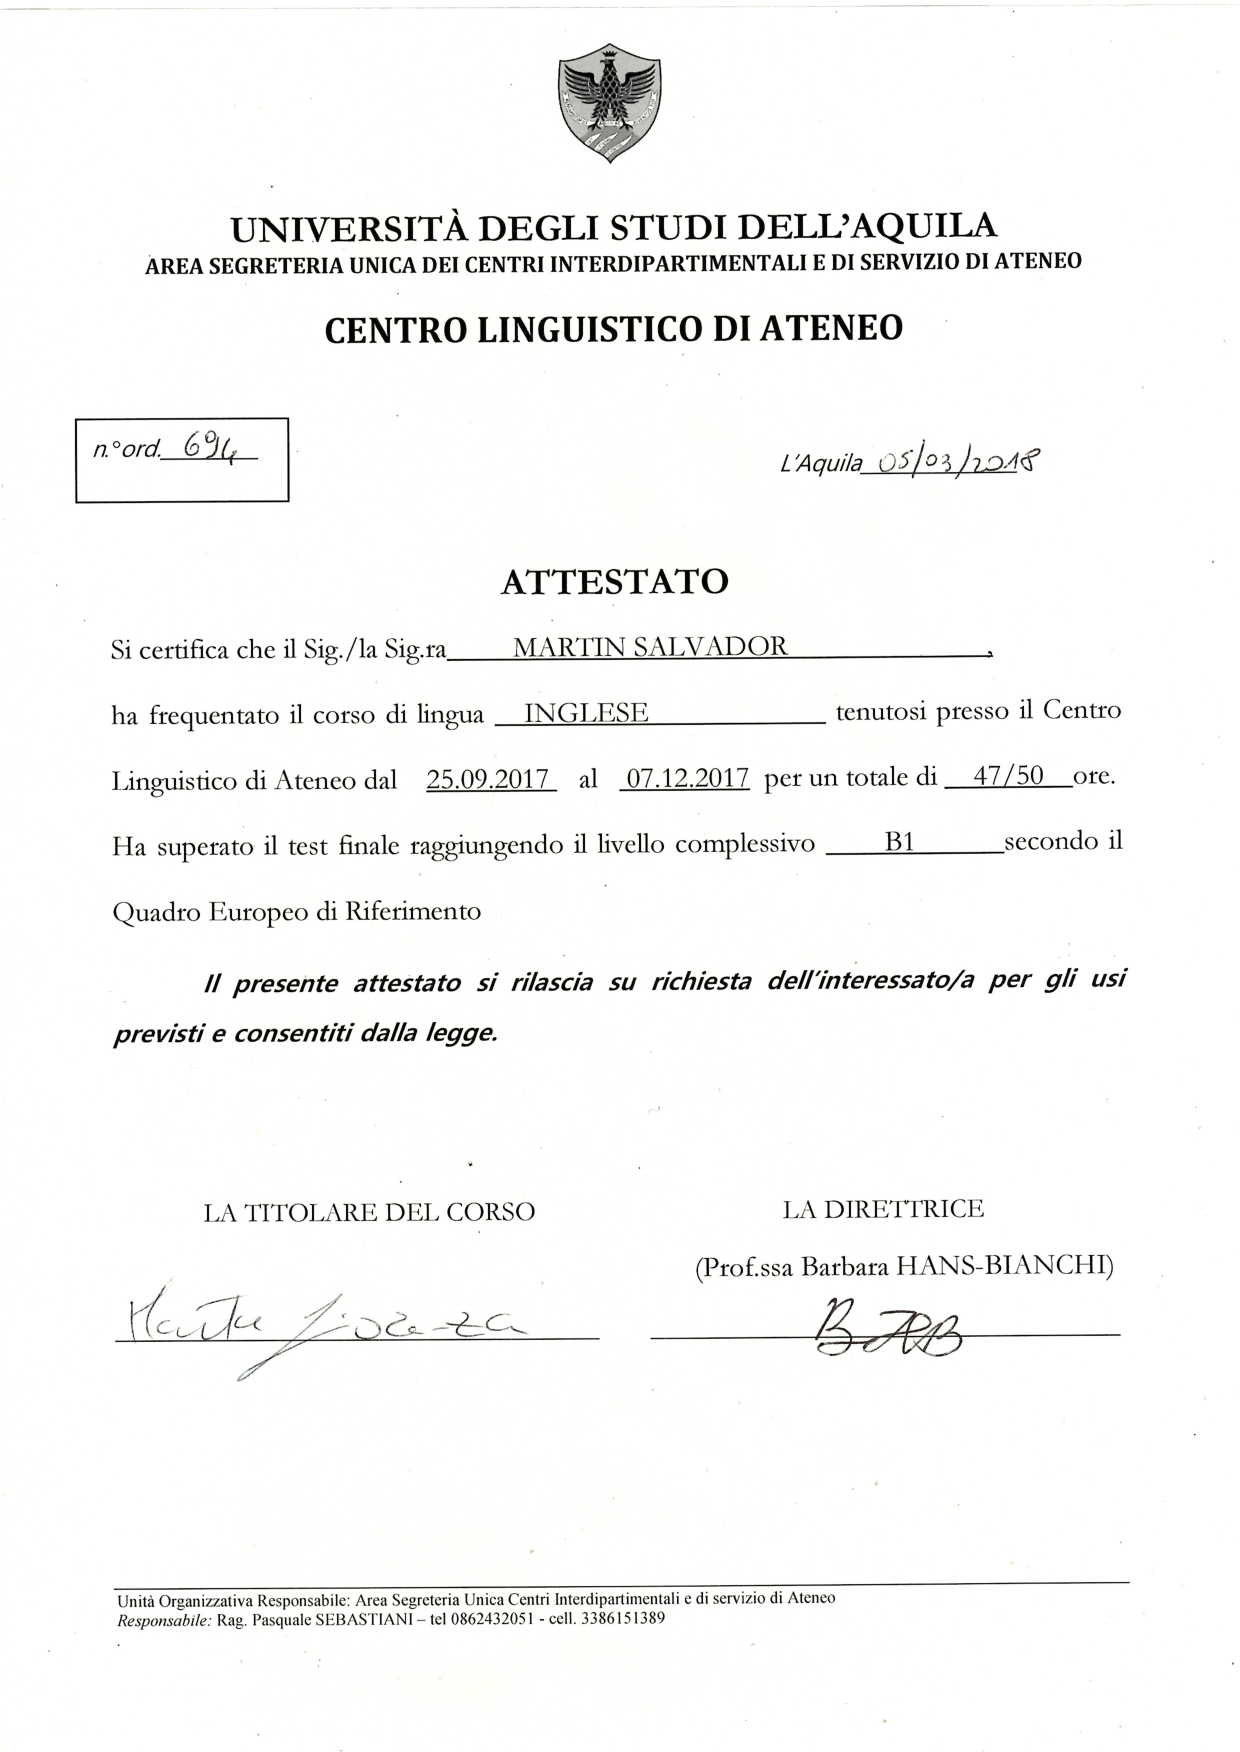
\includepdf{English(it)}
  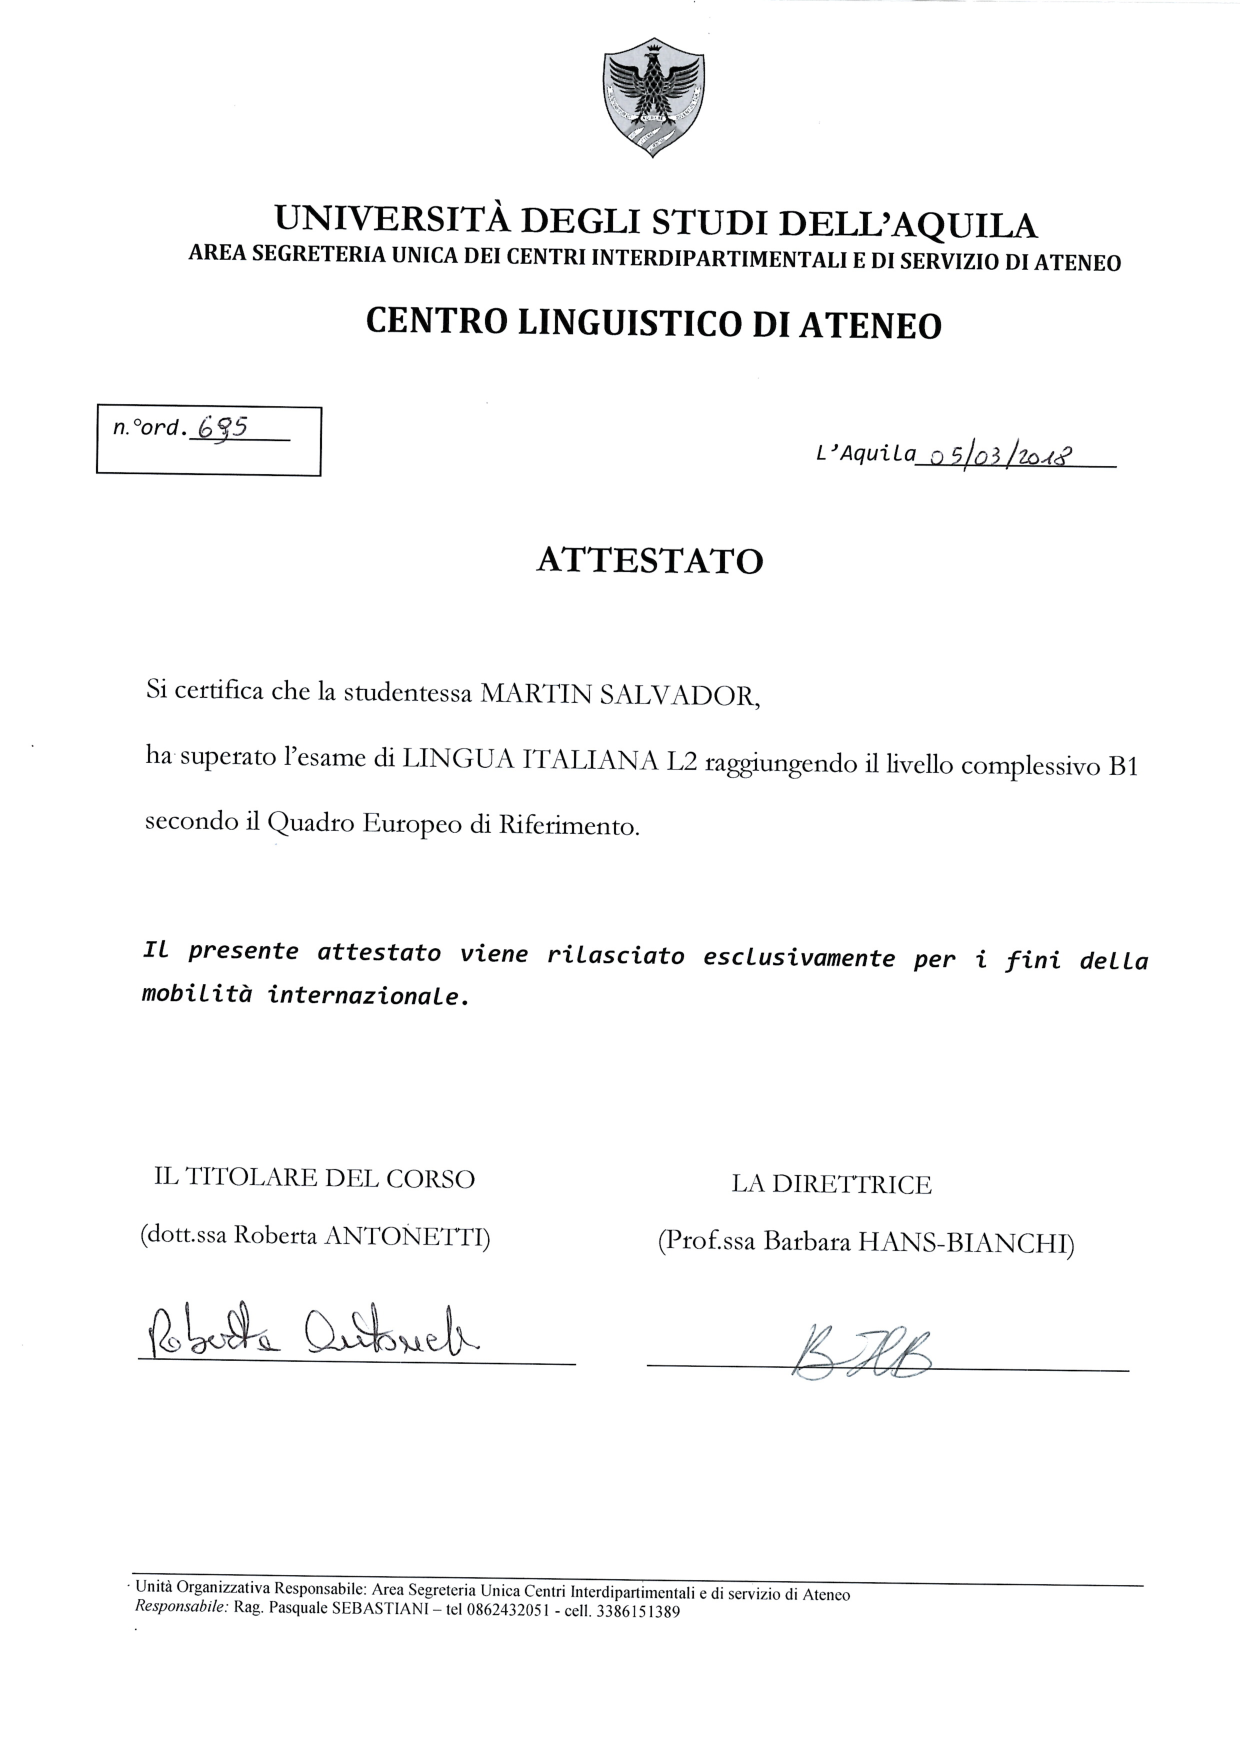
\includepdf{Italian(it)}
  \end{europasscv}

\end{document}